%%%%%%%%%%%%%%%%%%%%%%%%%%%%%%%%%%%%%%%%%
% fphw Assignment
% LaTeX Template
% Version 1.0 (27/04/2019)
%
% This template originates from:
% https://www.LaTeXTemplates.com
%
% Authors:
% Class by Felipe Portales-Oliva (f.portales.oliva@gmail.com) with template 
% content and modifications by Vel (vel@LaTeXTemplates.com)
%
% Template (this file) License:
% CC BY-NC-SA 3.0 (http://creativecommons.org/licenses/by-nc-sa/3.0/)
%
%%%%%%%%%%%%%%%%%%%%%%%%%%%%%%%%%%%%%%%%%

%----------------------------------------------------------------------------------------
%	PACKAGES AND OTHER DOCUMENT CONFIGURATIONS
%----------------------------------------------------------------------------------------

\documentclass[
	12pt, % Default font size, values between 10pt-12pt are allowed
	%letterpaper, % Uncomment for US letter paper size
	%spanish, % Uncomment for Spanish
]{fphw}

% Template-specific packages
\usepackage[utf8]{inputenc} % Required for inputting international characters
\usepackage[T1]{fontenc} % Output font encoding for international characters
\usepackage{mathpazo} % Use the Palatino font

\usepackage{graphicx} % Required for including images
\usepackage{amsmath}
\usepackage{booktabs} % Required for better horizontal rules in tables

\usepackage{listings} % Required for insertion of code
\usepackage{longtable,booktabs}
\usepackage{enumerate} % To modify the enumerate environment
%codes setting
\RequirePackage{listings}
\RequirePackage{xcolor}
\definecolor{dkgreen}{rgb}{0,0.6,0}
\definecolor{gray}{rgb}{0.5,0.5,0.5}
\definecolor{mauve}{rgb}{0.58,0,0.82}
\lstset{
	numbers=left,  
	frame=tb,
	aboveskip=3mm,
	belowskip=3mm,
	showstringspaces=false,
	columns=flexible,
	framerule=1pt,
	rulecolor=\color{gray!35},
	backgroundcolor=\color{gray!5},
	basicstyle={\ttfamily},
	numberstyle=\tiny\color{gray},
	keywordstyle=\color{blue},
	commentstyle=\color{dkgreen},
	stringstyle=\color{mauve},
	breaklines=true,
	breakatwhitespace=true,
	tabsize=3,
}
%----------------------------------------------------------------------------------------
%	ASSIGNMENT INFORMATION
%----------------------------------------------------------------------------------------

\title{Homework \#4} % Assignment title

\author{Hang Chen} % Student name


\institute{Boise State University \\ Department of geoscience} % Institute or school name

\class{GEOS 422 / GEOPH 522: Data Analysis and Geostatistics} % Course or class name


%----------------------------------------------------------------------------------------

\begin{document}

\maketitle % Output the assignment title, created automatically using the information in the custom commands above

%----------------------------------------------------------------------------------------
%	ASSIGNMENT CONTENT
%----------------------------------------------------------------------------------------

\section*{Question 1}

\begin{problem}
Subdivide the data into 4 different continuous sections (each 200 meters long) , calculate
summary statistics and plot the relative density histogram and kernel pdf of the accumulation
rates in each section.

\end{problem}




%------------------------------------------------

\subsection*{Answer}
In this question, I use the myfun.m function to get the kernel pdf of the accumulation rates.

The plot

\begin{figure}[htbp]
	\centering
	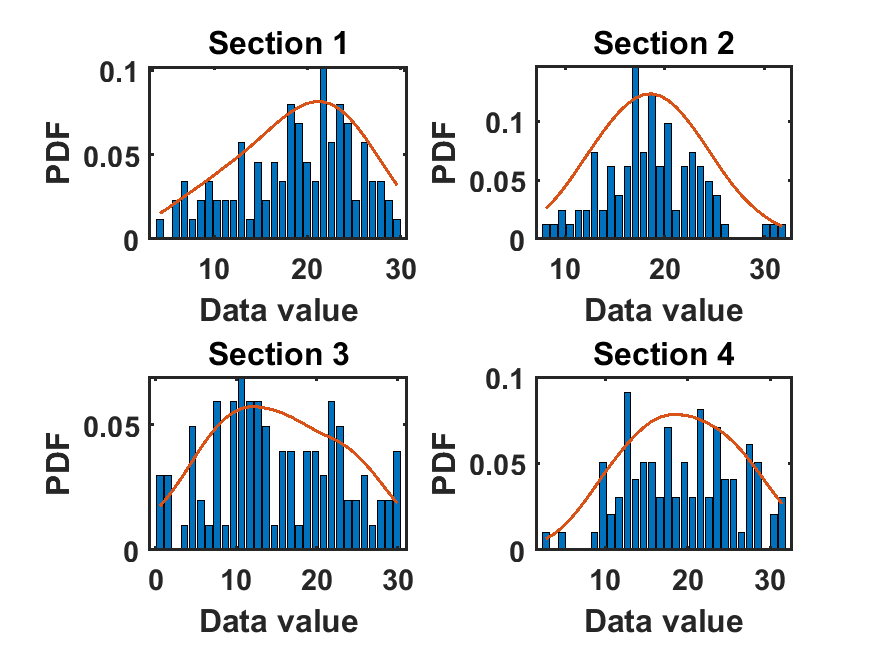
\includegraphics[width=1\columnwidth]{Q1.png} 
	\caption{Relative density histogram and kernel pdf of the accumulation
		rates in each section}
\end{figure}

The codes


\begin{lstlisting}[language=Matlab,escapeinside=``]
part1_x=x(1:100); %get the first section for x
part1_y=y(1:100); %get the first section for y
mean1(1)=mean(part1_y) % calculate the mean for part 1
std1(1)=std(part1_y) % calculate the standard deviation for part 1

part2_x=x(101:200);%get the second section for x
part2_y=y(101:200);%get the second section for y
mean1(2)=mean(part2_y) % calculate the mean for part 2
std1(2)=std(part2_y)% calculate the standard deviation for part 2

part3_x=x(201:300);%get the third section for x
part3_y=y(201:300);%get the third section for y
mean1(3)=mean(part3_y)% calculate the mean for part 3
std1(3)=std(part3_y)% calculate the standard deviation for part 3

part4_x=x(301:400);%get the fourth section for x
part4_y=y(301:400);%get the fourth section for y
mean1(4)=mean(part4_y)% calculate the mean for part 4
std1(4)=std(part4_y)% calculate the standard deviation for part 4

bins=30;
h=10;% window size for Kernel esimate

figure(1)
subplot(2,2,1)% for section 1
[centers] =plotRDH(part1_y,bins);%relative density histogram
hold on
[f] = myfun(part1_y,centers,h); % do the Kernel estimation 
plot(centers,f,'LineWidth',1.5)  % plot the Kernel estimation 
title('Section 1')
set(gca,'LineWidth',1,'FontSize',14,'FontWeight','bold')

subplot(2,2,2)% for section 2
[centers] =plotRDH(part2_y,bins);%relative density histogram
hold on
[f] = myfun(part2_y,centers,h); % do the Kernel estimation 
plot(centers,f,'LineWidth',1.5)  % plot the Kernel estimation 
title('Section 2')
set(gca,'LineWidth',1,'FontSize',14,'FontWeight','bold')

subplot(2,2,3)% for section 3
[centers] =plotRDH(part3_y,bins);%relative density histogram
hold on
[f] = myfun(part3_y,centers,h); % do the Kernel estimation 
plot(centers,f,'LineWidth',1.5)  % plot the Kernel estimation 
title('Section 3')
set(gca,'LineWidth',1,'FontSize',14,'FontWeight','bold')

subplot(2,2,4)% for section 4
[centers] =plotRDH(part4_y,bins);%relative density histogram
hold on
[f] = myfun(part4_y,centers,h); % do the Kernel estimation 
plot(centers,f,'LineWidth',1.5)  % plot the Kernel estimation 
title('Section 4')
set(gca,'LineWidth',1,'FontSize',14,'FontWeight','bold')
print('Q1','-dpng')


\end{lstlisting}


 myfun.m function
 \begin{lstlisting}[language=Matlab,escapeinside=``]
 function [f] = myfun(D,x0,h)
 % it is used to generate kernel density estimate
 % input D is the data, x0 is the central points and h is windows length

 for n=1:length(x0)
 dist=(D-x0(n)); % distance from x0 to all data values
 Ix=find(abs(dist)<h); % finding all datapoints  within h of x0
 w=15/16*(1-(dist(Ix)/h).^2).^2; % weights for all datapoints within h of x0
 f(n)=nansum(w); % sum the weights
 end
 dx=nanstd(D)/10;
 f=1/sum(f*dx)*f; % normalized PDF so that it integrates to 1
 end
\end{lstlisting}
%----------------------------------------------------------------------------------------

\section*{Question 2}

\begin{problem}
Are the first two basic assumptions of second order stationarity approximately correct (i.e.
constant mean, constant variance)?
	
\end{problem}

%------------------------------------------------

\subsection*{Answer}

From the question 1, I get the mean and standard deviation to the four section data. The mean for the four sections are 18.8511, 18.6016, 15.1174 and 19.2627. The standard deviation for the four sections are 6.2728, 4.6491, 7.9478 and 6.4698. 

It seems both the mean and standard deviation of four sections are not the same and not very close. Therefore, two basic assumptions of second order stationarity is not correct but not very far away.

%----------------------------------------------------------------------------------------

\section*{Question 3}

\begin{problem}
Calculate the semivariance, covariance, and autocorrelation and plot.
\end{problem}

%------------------------------------------------

\subsection*{Answer} 

The relationship among semivariance, covariance, and autocorrelation is that 

\begin{equation}
	\gamma(h)=C(0)-C(h),
\end{equation}
where C is the covariance  and $\gamma$ is the semivariance.

Then it can be converted into

\begin{equation}
\gamma(h)=\sigma^2(1-\rho(h)),	
\end{equation}
where the $\sigma$ is the varance and $\rho$ is the autocorrelation.

Therefore, in this question, first I get the semivariance by using semivariogram.m function. Then after calculating the variance, I can calculate the covariance by equation (1). Finally, I can obtain the autocorrelation by equation (2), or in short using the covariacne over the variacne.


\begin{figure}[htbp]
	\centering
	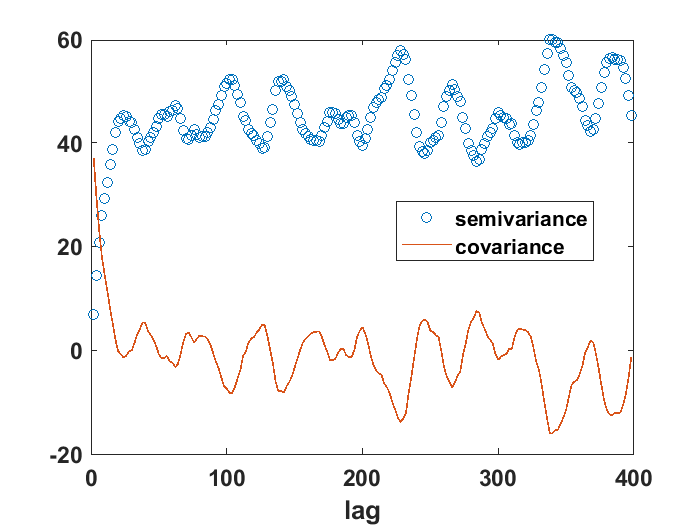
\includegraphics[width=0.68\columnwidth]{Q3_1.png} 
	\caption{The plot for the semivariance and covariance.}
\end{figure}

\begin{figure}[htbp]
	\centering
	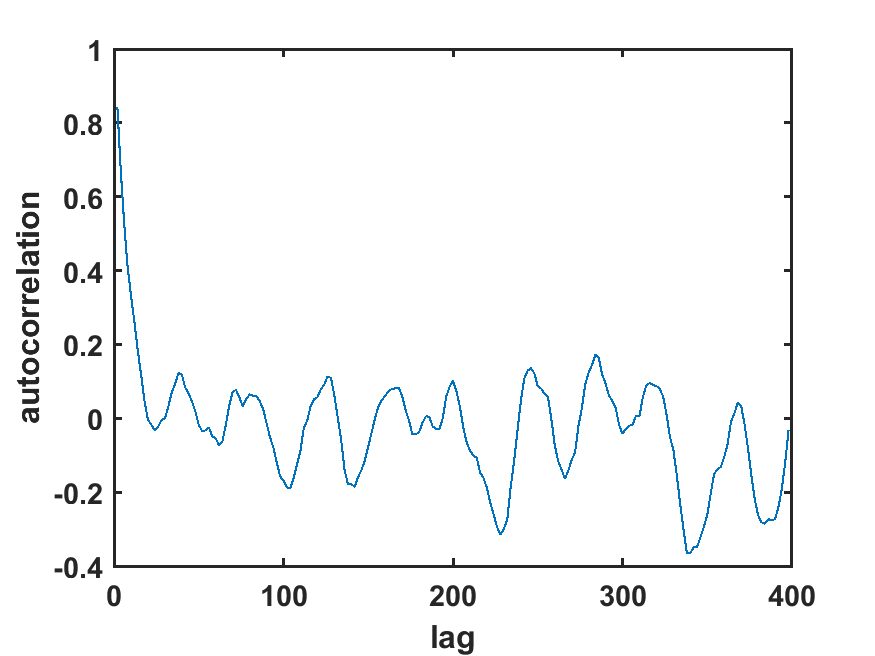
\includegraphics[width=0.68\columnwidth]{Q3_2.png} 
	\caption{The plot for the autocorrelation.}
\end{figure}


The codes

\begin{lstlisting}[language=Matlab,escapeinside=``]
[h,V] = semivariogram(x,y);% get the semivariance

var_data=var(y); %calculate the variance
cov_data=var_data-V; %calculate the covariance

auto_data=cov_data./var_data;%calculate the autocorrelation

figure(2); clf
plot(h,V,'o')%plot the semivariance
hold on
plot(h,cov_data,'linewidth',1)%plot the covariance
xlabel('lag')
legend('semivariance','covariance')
set(gca,'LineWidth',1,'FontSize',14,'FontWeight','bold')
print('Q3_1','-dpng')
figure(3)
plot(h,auto_data,'linewidth',1)%plot the autocorrelation
xlabel('lag')
ylabel('autocorrelation')
set(gca,'LineWidth',1,'FontSize',14,'FontWeight','bold')
print('Q3_2','-dpng')
\end{lstlisting}

semivariogram.m

\begin{lstlisting}[language=Matlab,escapeinside=``]
function [h,V] = semivariogram(x,y)
% simple 1D semivariogram function for equally spaced data
% INPUT:  
%  x = distance vector
%  y = measurement vector
% OUTPUT:
%  h = lag distance
%  V = semivariogram result
% SNTX: [h,V] = semivariogram(x,y)

% first define the lags
dx=mean(diff(x)); % average spacing
extent=(max(x)-min(x)); % extent
N=length(x); % number of data points
h=dx:dx:extent/2; % lags - only calculating to 1/2 extent to avoid bias
npairs=zeros(length(h),1); % preallocate number of pairs
V=zeros(length(h),1); % preallocate semivariance
for q=1:length(h) % loop over lags
npairs(q)=N-q; % number of pairs at each lag
Iu=1:(N-q); % index to heads
Iv=(q+1):N; % index to tails
V(q)=1/(2*npairs(q))*sum((y(Iu)-y(Iv)).^2); % semivariance
end 
\end{lstlisting}
%----------------------------------------------------------------------------------------
\clearpage
\section*{Question 4 }

\begin{problem}
Using Monte-Carlo simulation, plot the uncertainty in semivariance for random samples of
the point pairs for a constant number of pairs of points, Np, at each lag. Show the uncertainty
for Np =10, 50, and 100 pairs of points.
\end{problem}

%------------------------------------------------

\subsection*{Answer}

In this question, I use the semivariogram\_mc2.m function to do the Monte-Carlo simulation and use the 95\% uncertainty limits on the semivariance.

\begin{figure}[htbp]
	\centering
	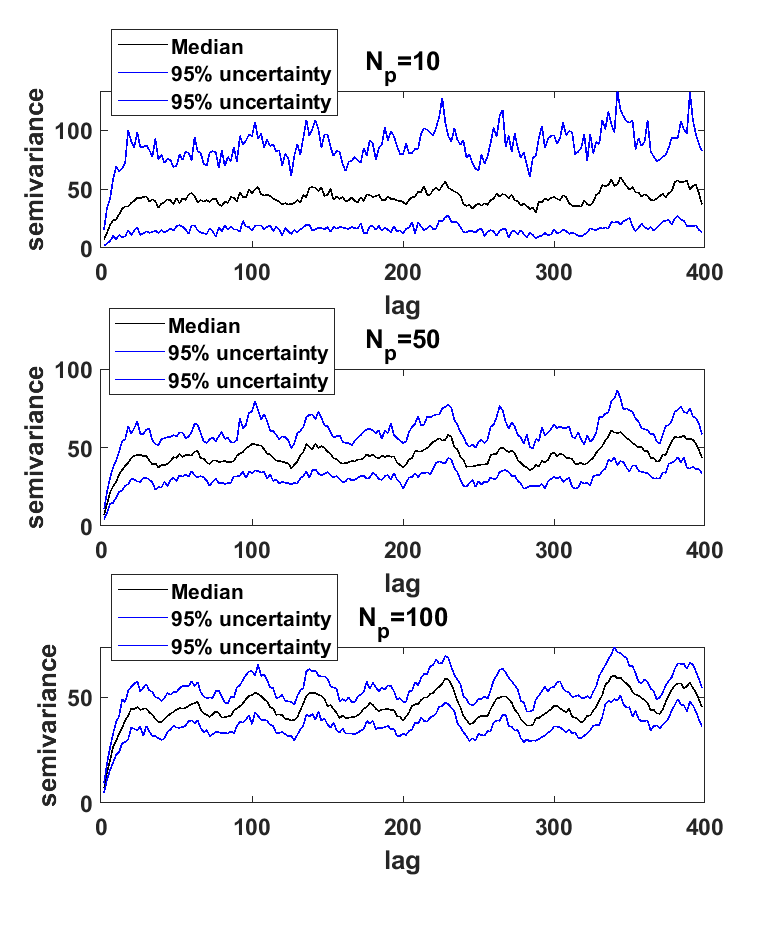
\includegraphics[width=0.7\columnwidth]{Q4.png} 
	\caption{Plot the mediam and the uncertainty
		for Np =10, 50, and 100 pairs of points.}
\end{figure}


The codes 

\begin{lstlisting}[language=Matlab,escapeinside=``]

np=10; % define the number of paris of points
[h1,V1,npairs1] = semivariogram_mc(x,y,np);% semivariance for 10 paris

np=50; % define the number of paris of points
[h2,V2,npairs2] = semivariogram_mc(x,y,np);% semivariance for 50 paris

np=100; % define the number of paris of points
[h3,V3,npairs3] = semivariogram_mc(x,y,np);% semivariance for 100 paris

figure(4)
subplot(3,1,1)
plot(h1,V1(:,2),'k','linewidth',1)% plot the median of semivariance for 10 paris
hold on
plot(h1,V1(:,1),'b','linewidth',1)% plot the 95% uncertainty limits of semivariance for 10 paris
hold on
plot(h1,V1(:,3),'b','linewidth',1)% plot the 95% uncertainty limits of semivariance for 10 paris
legend('Median','95% uncertainty','95% uncertainty')
xlabel('lag')
ylabel('semivariance')
title('N_p=10')
set(gca,'LineWidth',1,'FontSize',14,'FontWeight','bold')

subplot(3,1,2)
plot(h2,V2(:,2),'k','linewidth',1)% plot the median of semivariance for 50 paris
hold on
plot(h2,V2(:,1),'b','linewidth',1)% plot the 95% uncertainty limits of semivariance for 50 paris
hold on
plot(h2,V2(:,3),'b','linewidth',1)% plot the 95% uncertainty limits of semivariance for 50 paris
legend('Median','95% uncertainty','95% uncertainty')
xlabel('lag')
ylabel('semivariance')
title('N_p=50')
set(gca,'LineWidth',1,'FontSize',14,'FontWeight','bold')

subplot(3,1,3)
plot(h3,V3(:,2),'k','linewidth',1)% plot the median of semivariance for 100 paris
hold on
plot(h3,V3(:,1),'b','linewidth',1)% plot the 95% uncertainty limits of semivariance for 100 paris
hold on
plot(h3,V3(:,3),'b','linewidth',1)% plot the 95% uncertainty limits of semivariance for 100 paris
legend('Median','95% uncertainty','95% uncertainty')
xlabel('lag')
ylabel('semivariance')
title('N_p=100')
set(gca,'LineWidth',1,'FontSize',14,'FontWeight','bold')
print('Q4','-dpng')

\end{lstlisting}

semivariogram\_mc2.m
\begin{lstlisting}[language=Matlab,escapeinside=``]
function [h,V,npairs] = semivariogram_mc2(x,y,np)
% simple 1D semivariogram function for equally spaced data
% INPUT:  
%  x = distance vector
%  y = measurement vector
%  np = number of pairs of points to use 
% OUTPUT:
%  h = lag distance
%  V = semivariogram result
% SNTX: [h,V,npairs] = semivariogram_mc(x,y,np)

% first define the lags
dx=mean(diff(x)); % average spacing
extent=(max(x)-min(x)); % extent
N=length(x); % number of data points
h=dx:dx:extent/2; % lags - only calculating to 1/2 extent to avoid bias
npairs=zeros(length(h),1); % preallocate number of pairs
V=zeros(length(h),3); % preallocate semivariance
for q=1:length(h) % loop over lags
npairs(q)=N-q; % number of pairs at each lag
Iu=1:(N-q); % index to heads
Iv=(q+1):N; % index to tails
Vt=zeros(10,1);
for m=1:100 % monte carlo for uncertainties
I2=randsample(Iu,np); % random sampling of pairs
Iut=Iu(I2);
Ivt=Iv(I2);
Vt(m)=1/(2*np)*sum((y(Iut)-y(Ivt)).^2); % semivariance
end
V(q,:)=quantile(Vt,[0.025 0.5 0.975]);
end 
\end{lstlisting}


%----------------------------------------------------------------------------------------
\clearpage
\section*{Question 5 }

\begin{problem}
Plot the semivariance for the 4 different equal continuous sections that you used above. Is
the third assumption of second order stationarity approximately correct (i.e. semivariance
depends only on the lag)?
\end{problem}

%------------------------------------------------

\subsection*{Answer}

In this question, I use semivariogram.m function to obtion the semivariance for the 4 different equal continuous sections. The results are shown in figure 5. From the figure 5, we can see that the four lines differ a lot, which means that third assumption of second order stationarity is not correct, because it seems that semivariance is not only
depends only on the lag. 


\begin{figure}[htbp]
	\centering
	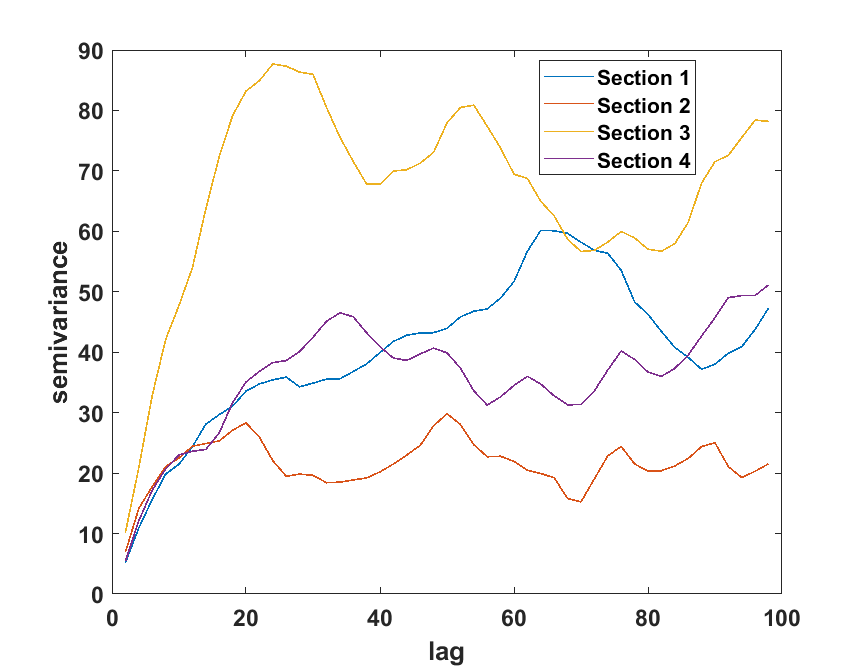
\includegraphics[width=0.8\columnwidth]{Q5.png} 
	\caption{Plot the semivariance for the 4 different equal continuous sections}
\end{figure}

The codes

\begin{lstlisting}[language=Matlab,escapeinside=``]

[h_part1,V_part1] = semivariogram(part1_x,part1_y);% semivariance for part 1

[h_part2,V_part2] = semivariogram(part2_x,part2_y);% semivariance for part 2

[h_part3,V_part3] = semivariogram(part3_x,part3_y);% semivariance for part 3

[h_part4,V_part4] = semivariogram(part4_x,part4_y);% semivariance for part 4

figure(5)

plot(h_part1,V_part1,'linewidth',1)%plot the semivariance for part 1
hold on
plot(h_part2,V_part2,'linewidth',1)%plot the semivariance for part 2
hold on
plot(h_part3,V_part3,'linewidth',1)%plot the semivariance for part 3
hold on
plot(h_part4,V_part4,'linewidth',1)%plot the semivariance for part 4
xlabel('lag')
ylabel('semivariance')
legend('Section 1','Section 2','Section 3','Section 4')
set(gca,'LineWidth',1,'FontSize',14,'FontWeight','bold')
print('Q5','-dpng')

\end{lstlisting}


\clearpage
\section*{Question 6 }

\begin{problem}
Using the experimental variogram for the entire dataset, fit a bounded linear model:
\begin{equation}
	\begin{aligned}
	\gamma(h) &=\frac{c h}{a} & & h \leq a \\
	&=c & & h>a
	\end{aligned}
\end{equation}
where c is the sill and a is the range. Do this using a brute-force method, by looping over a
range of values of c and a.

\end{problem}

\subsection*{Answer}

Through brute force method, I get the optimum a=17 and c=46;

\begin{figure}[htbp]
	\centering
	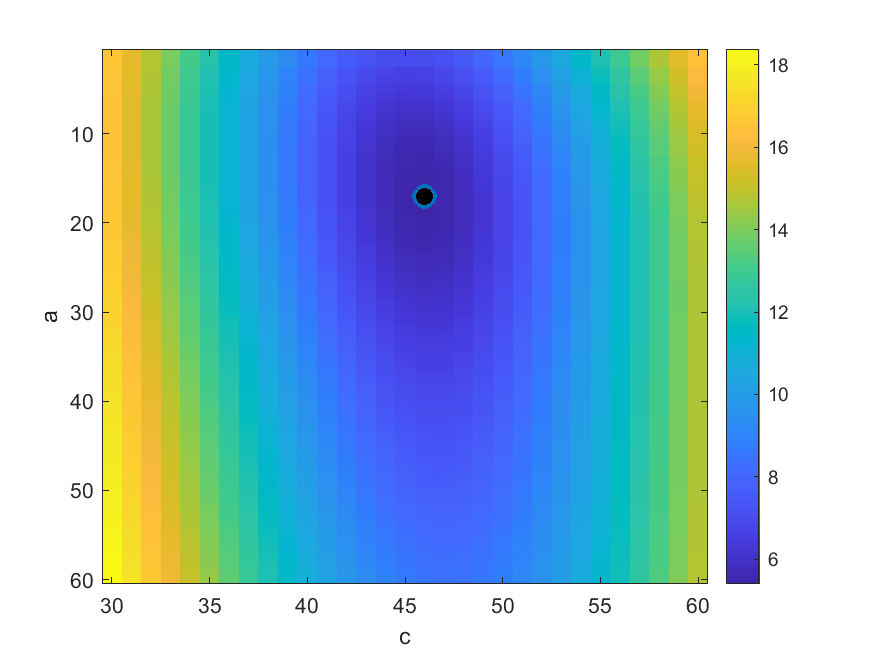
\includegraphics[width=0.8\columnwidth]{Q6.png} 
	\caption{The RMSE image}
\end{figure}

\begin{lstlisting}[language=Matlab,escapeinside=``]
% brute force approach

a=1:60; %brute force range for a
c=30:60; %brute force range for c
rmse=zeros(length(a),length(c)); %intial rmse

for n=1:length(a)
for m=1:length(c)
rmse(n,m)=model_variogram_error(h,V,c(m),a(n),'L'); % calculate RMSE for the all a and c
end
end

figure(6);clf
imagesc(c,a,rmse);% image the rmse
xlabel('c')
ylabel('a')
colorbar
minvalue=min(min(rmse)) %find minimum RMSE
[abestindex,cbeatindex]=find(rmse==minvalue);%find index of minimum RMSE

abest=a(abestindex) %the optimum a in brute force method
cbest=c(cbeatindex) %the optimum c in brute force method
hold on
plot(cbest,abest,'o','MarkerSize',10,'MarkerFaceColor','k','linewidth',2); % plot the best point in image

print('Q6','-dpng')


\end{lstlisting} 



%----------------------------------------------------------------------------------------



\section*{Question 7}

\begin{problem}
Repeat using the MATLAB function fminsearch.m to find the best parameters.	
\end{problem}


\subsection*{Answer}
In this question, I use the function model\_variogram\_error.m.
The results from fminsearch.m are best a=16.9598 and c=45.8883.


The codes
\begin{lstlisting}[language=Matlab,escapeinside=``]

fh=@(p)model_variogram_error(h,V,p(1),p(2),'L');%function handle
[pbest,fval]=fminsearch(fh,[30,60]);%gradient descent method to find best parameters

\end{lstlisting}
model\_variogram\_error.m

\begin{lstlisting}[language=Matlab,escapeinside=``]

function rmse=model_variogram_error(h,V,c,a,type)
% variogram using the bounded linear and spherical models
% HPM 11/3/2020
% INPUT:
% h = lags for modeled estimates
% V = experimental variogram estimate
% c = variogram sill
% a = variogram range
% type = 'L' for linear and 'S' for spherical

Ix=find(h<=a); % finding lags less than a
switch type
case 'L'
Vm(Ix)=c*h(Ix)/a; % bounded linear
case 'S'
Vm(Ix)=c*(3*h(Ix)/(2*a)-0.5*(h(Ix)/a).^3); % spherical model
end

Ix2=h>a; % lags greater than range
Vm(Ix2)=c; % set equal to sill
V=V(:); Vm=Vm(:);
rmse=sqrt(mean((Vm-V).^2)); % root mean squared error

\end{lstlisting}

\section*{Question 8 }

\begin{problem}
Using fminsearch.m, fit a spherical model to the experimental variogram:
\begin{equation}
	\begin{array}{rlr}
	\gamma(h) & =c\left(\frac{3 h}{2 a}-\frac{h^{3}}{2 a^{3}}\right) & h \leq a \\
	& =c
	\end{array}
\end{equation}
\end{problem}


\subsection*{Answer}


The results from fminsearch.m are best a=16.5052 and c=45.9071.

The codes

\begin{lstlisting}[language=Matlab,escapeinside=``]
fh=@(p)model_variogram_error(h,V,p(1),p(2),'S');%function handle
[pbest1,fval1]=fminsearch(fh,[30,60]);%gradient descent method to find best parameters

\end{lstlisting}




\section*{Question 9 }

\begin{problem}
Add a nugget to the model and repeat.
	
\end{problem}

\subsection*{Answer}
In this question, I define a new function model\_variogram\_error\_withnugget.m, which helps calculate the RMSE with nugget.

In linear model, the best a=18.9239, c=39.9159, and nugget=6.5935.

In spherical model, the best a=24.0303, c=42.0462, and nugget=3.8732.

The codes
 \begin{lstlisting}[language=Matlab,escapeinside=``]
%for linear model

% first use brute force approach to find a suitable intital guess
a=1:60;%brute force range for a
c=30:60;%brute force range for c
n=0:10;%brute force range for n
for i=1:length(a)
for j=1:length(c)
for k=1:length(n)
RMSE_3d(i,j,k)=model_variogram_error_withnugget(h,V,c(j),a(i),n(k),'L');% calculate RMSE for the all a, c and n
end
end
end

%find the min RMSE and regarding index
[min_val, position_min] = min(RMSE_3d(:)); 
[abestindex1,cbeatindex1,nbestindex1] = ind2sub(size(RMSE_3d),position_min);

abest1=a(abestindex1)%the optimum a in brute force method
cbest1=c(cbeatindex1)%the optimum c in brute force method
nbest1=n(nbestindex1)%the optimum n in brute force method

%for linear model
fh=@(p)model_variogram_error_withnugget(h,V,p(1),p(2),p(3),'L');%function handle
[pbest_3d,fval2]=fminsearch(fh,[cbest1,abest1,nbest1]);%gradient descent method to find best parameters

%for spherical model

% first use brute force approach to find a suitable intital guess
a=1:60;%brute force range for a
c=30:60;%brute force range for c
n=0:10;%brute force range for n

for i=1:length(a)
for j=1:length(c)
for k=1:length(n)

RMSE_3d1(i,j,k)=model_variogram_error_withnugget(h,V,c(j),a(i),n(k),'S');% calculate RMSE for the all a, c and n
end
end
end

%find the min RMSE and regarding index
[min_val, position_min] = min(RMSE_3d1(:)); 
[abestindex2,cbeatindex2,nbestindex2] = ind2sub(size(RMSE_3d1),position_min);

abest2=a(abestindex2)%the optimum a in brute force method
cbest2=c(cbeatindex2)%the optimum c in brute force method
nbest2=n(nbestindex2)%the optimum n in brute force method

%for spherical model
fh=@(p)model_variogram_error_withnugget(h,V,p(1),p(2),p(3),'S');%function handle
[pbest_3d1,fval3]=fminsearch(fh,[cbest2,abest2,nbest2]);%gradient descent method to find best parameters

\end{lstlisting}
 
model\_variogram\_error\_withnugget.mmodel\_variogram\_error\_withnugget.m  

 \begin{lstlisting}[language=Matlab,escapeinside=``]
 
function rmse=model_variogram_error_withnugget(h,V,c,a,n,type)
% variogram using the bounded linear and spherical models
% HPM 11/3/2020
% INPUT:
% h = lags for modeled estimates
% V = experimental variogram estimate
% c = variogram sill
% a = variogram range
% n = nugget
% type = 'L' for linear and 'S' for spherical

Ix=find(h<=a); % finding lags less than a
switch type
case 'L'
Vm(Ix)=c*h(Ix)/a+n; % bounded linear
case 'S'
Vm(Ix)=c*(3*h(Ix)/(2*a)-0.5*(h(Ix)/a).^3)+n; % spherical model
end

Ix2=h>a; % lags greater than range
Vm(Ix2)=c+n; % set equal to sill
V=V(:); Vm=Vm(:);
rmse=sqrt(mean((Vm-V).^2)); % root mean squared error

\end{lstlisting}

\clearpage
 
 \section*{Question 10 }
 
 \begin{problem}
Plot all 4 variogram models along with the experimental variogram.
 	
 \end{problem}
 
 \subsection*{Answer}
 In this question, I firstly plot four models and the experimental variogram in one figure, but it cannot be seen very clear. Therefore, I also provide a version includes four figures.
 
 \begin{figure}[htbp]
	\centering
	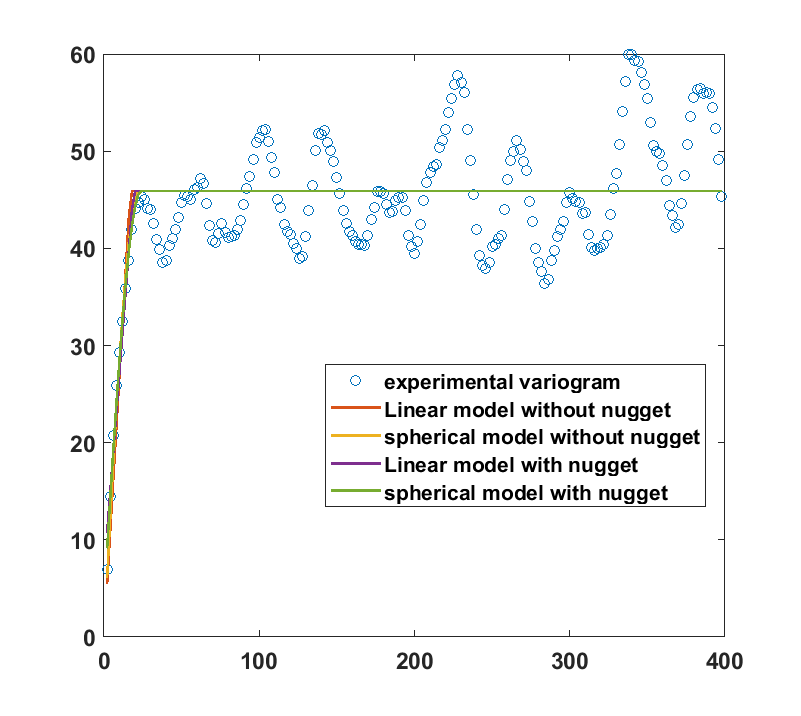
\includegraphics[width=0.6\columnwidth]{Q10_1.png} 
	\caption{Plot all 4 variogram models along with the experimental variogram in a figure }
\end{figure}
 

 \begin{figure}[htbp]
 	\centering
 	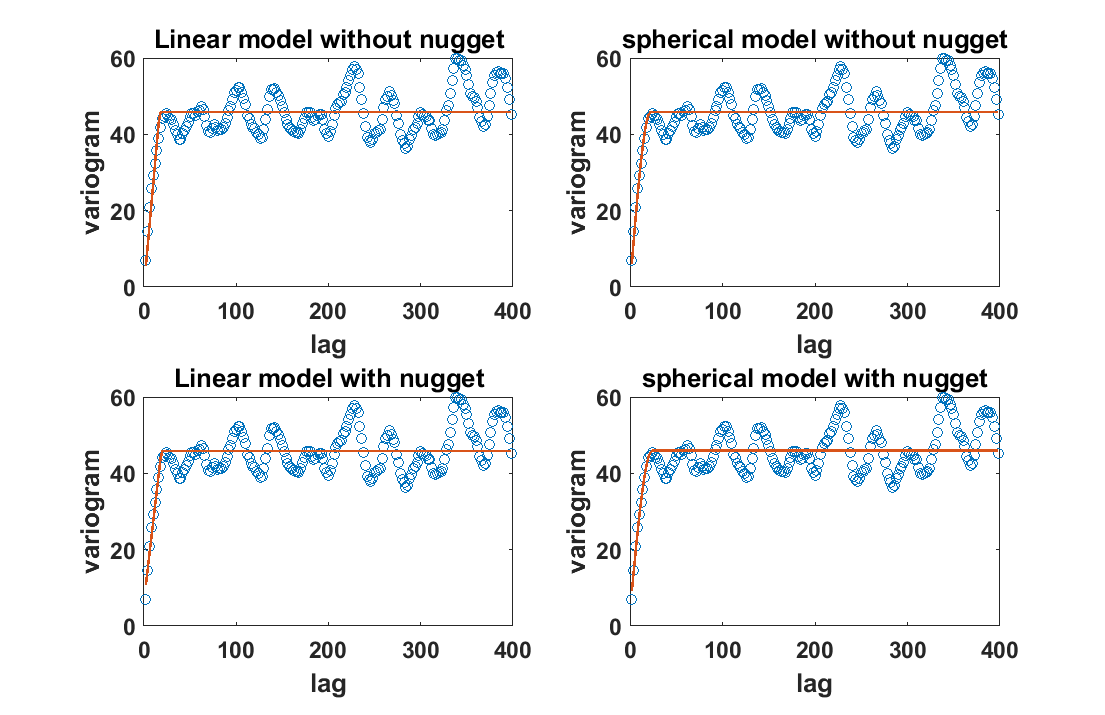
\includegraphics[width=0.68\columnwidth]{Q10_2.png} 
 	\caption{Plot all 4 variogram models along with the experimental variogram in four figures }
 \end{figure}
 
The codes
 
  \begin{lstlisting}[language=Matlab,escapeinside=``]

pTrain=0.9;%define the pecent that's used in polynomial fit
nMC=1000; %times for Monte-Carlo
rmseCV2=zeros(nMC,1); % initializing
u1=vel(1);

for p=1:nMC
[trainset, ~] = getTrainTest([depth vel],pTrain);%get 90% data
ztrain=trainset(:,1); % depths for training
vtrain=trainset(:,2); % velocity for training
fh=@(A)physics1(ztrain,vtrain,u1,A); % function handle, A can be tuned to data in v,z
A0=Abest(1);% initial guess of A
[Abest1,fval1] = fminsearch(fh,A0); %find the best parameters, and get the error
Aall(p)=Abest1;% store the A
rmseCV2(p)=fval1;% store the RMSE
end

bins=30;
figure
subplot(1,2,1)
plotRDH(Aall,bins);
title('A')
set(gca,'LineWidth',1,'FontSize',14,'FontWeight','bold')
subplot(1,2,2)
plotRDH(rmseCV2,bins);
title('RMSE')
set(gca,'LineWidth',1,'FontSize',14,'FontWeight','bold')
print('Q10','-dpng')

 \end{lstlisting}
 
 
 

\clearpage
 \section*{Question 11 }

\begin{problem}

Choose your best variogram model from the 4 above. Using 100 Monte-carlo simulations, fit the model using 50 point pairs at each lag, using fminsearch.m.
	
\end{problem}

\subsection*{Answer}

In this question, I define function semivariogram\_mc\_model.m to do the Monte-Carlo simulations. At first, I compare the RMSE for different models. 

\begin{itemize}
	\item For the linear model without nugget, the RMSE=5.4001
	\item For the spherical model without nugget, the RMSE=5.3661
	\item For the linear model with nugget, the RMSE=5.3696
	\item For the spherical model with nugget, the RMSE=5.3571
\end{itemize}

It seems the spherical model with nugget has the smallest RMSE, so I choose this model for the follwing work.




The codes

\begin{lstlisting}[language=Matlab,escapeinside=``]
%choose the spherical model with nugget which has smallest RMSE
np=50;%define the np
[h,psave,Vsave] = semivariogram_mc_model(x,y,np);%using new function to obtain the best parameters and variogram results
\end{lstlisting}

\textbf{function semivariogram\_mc\_model.m}
                                                                                                                        
\begin{lstlisting}[language=Matlab,escapeinside=``]                                                                     
function [h,p,Vsave] = semivariogram_mc_model(x,y,np)
% simple 1D semivariogram function for equally spaced data
% INPUT:
%  x = distance vector
%  y = measurement vector
%  np = number of pairs of points to use
% OUTPUT:
%  h = lag distance
%  p = best parameters
%  Vsave = semivariogram result
% SNTX: [h,p,Vsave] = semivariogram_mc_model(x,y,np)

% first define the lags
dx=mean(diff(x)); % average spacing
extent=(max(x)-min(x)); % extent
N=length(x); % number of data points
h=dx:dx:extent/2; % lags - only calculating to 1/2 extent to avoid bias
npairs=zeros(length(h),1); % preallocate number of pairs
%V=zeros(length(h),3); % preallocate semivariance
% Vt=zeros(length(q),100);
for q=1:length(h) % loop over lags
npairs(q)=N-q; % number of pairs at each lag
Iu=1:(N-q); % index to heads
Iv=(q+1):N; % index to tails

for m=1:100 % monte carlo for uncertainties
I2=randsample(Iu,np); % random sampling of pairs
Iut=Iu(I2);
Ivt=Iv(I2);
Vt(q,m)=1/(2*np)*sum((y(Iut)-y(Ivt)).^2); % semivariance
end

end

for m=1:100
%for spherical model
% first use brute force approach to find a suitable intital guess
a=1:60;%brute force range for a
c=0:60;%brute force range for c
n=0:10;%brute force range for n

for i=1:length(a)
for j=1:length(c)
for k=1:length(n)
RMSE_3d1(i,j,k)=model_variogram_error_withnugget(h,Vt(:,m),c(j),a(i),n(k),'S');% calculate RMSE for the all a, c and n
end
end
end
%find the min RMSE and regarding index
[min_val, position_min] = min(RMSE_3d1(:));
[abestindex2,cbeatindex2,nbestindex2] = ind2sub(size(RMSE_3d1),position_min);

abest2=a(abestindex2);%the optimum a in brute force method
cbest2=c(cbeatindex2);%the optimum c in brute force method
nbest2=n(nbestindex2);%the optimum n in brute force method



fh=@(p)model_variogram_error_withnugget(h,Vt(:,m),p(1),p(2),p(3),'S');%function handle

%The below method
%    [pbest fval ef]=fmincon(fh,[cbest2,abest2,nbest2],[],[],[],[],[min(h),min(Vt(:,m)),min(Vt(:,m))],[max(h) max(Vt(:,m)) max(Vt(:,m))]);
[pbest,fval3]=fminsearch(fh,[cbest2,abest2,nbest2]);%gradient descent method to find best parameters
p(m,1:3)=pbest;%store the best parameters
V=model_variogram_withnugget(h,pbest(1),pbest(2),pbest(3),'S');
Vsave(m,1:length(h))=V;%store the model variogram
% to test the plot
%     plot(h,Vt(:,m),'o')
%     hold on
%     plot(h,V)
%   %   text('c=21019900,a=1741897013,n=4.27')
%     set(gca,'LineWidth',1,'FontSize',14,'FontWeight','bold')

end

\end{lstlisting}




 \section*{Question 12 }

\begin{problem}
Plot the experimental variogram with the median modeled variogram at each lag and 95\%
uncertainty limits on the modeled variogram, from your 100 variogram models.	
\end{problem}

\subsection*{Answer}

 \begin{figure}[htbp]
	\centering
	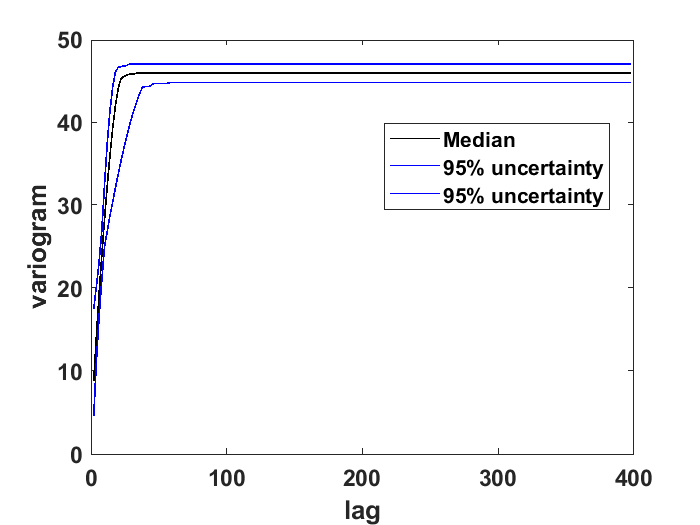
\includegraphics[width=0.8\columnwidth]{Q11.png} 
	\caption{Plot the experimental variogram with the median modeled variogram at each lag and 95\%
		uncertainty limits on the modeled variogram }
\end{figure}

The codes

\begin{lstlisting}[language=Matlab,escapeinside=``]
Vall=quantile(Vsave,[0.025 0.5 0.975]);% getmedian modeled variogram at each lag and 95% uncertainty limits
figure(9)
plot(h,Vall(2,:),'k','linewidth',1)% plot the median of semivariance 
hold on
plot(h,Vall(1,:),'b','linewidth',1)% plot the 95% uncertainty limits of semivariance
hold on
plot(h,Vall(3,:),'b','linewidth',1)% plot the 95% uncertainty limits of semivariance 
xlabel('lag')
ylabel('variogram')
legend('Median','95% uncertainty','95% uncertainty')
set(gca,'LineWidth',1,'FontSize',14,'FontWeight','bold')
print('Q11','-dpng')
\end{lstlisting}


 \section*{Question 13 }

\begin{problem}
Plot the relative density histogram and kernel pdf for each of the variogram model parameters (sill, range, and nugget).	
\end{problem}

\subsection*{Answer}

 \begin{figure}[htbp]
	\centering
	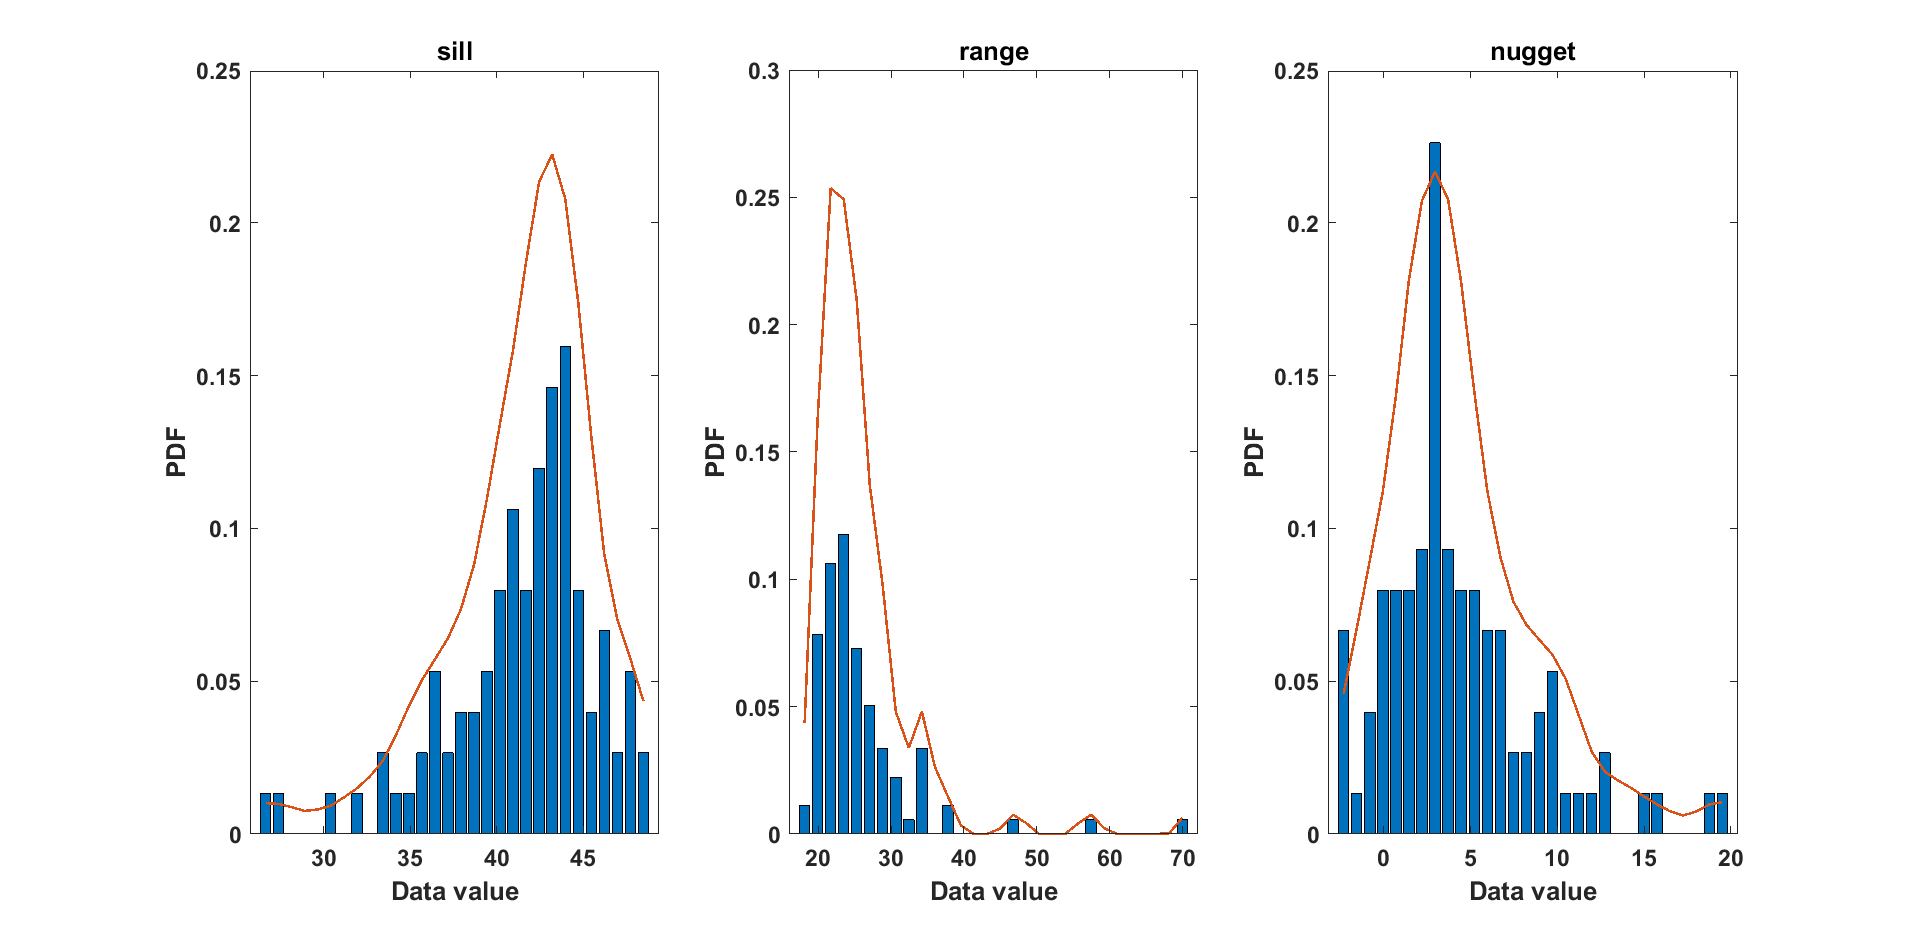
\includegraphics[width=1\columnwidth]{Q13.png} 
	\caption{Plot the relative density histogram and kernel pdf for each of the variogram model parameters (sill, range, and nugget). }
\end{figure}


\begin{lstlisting}[language=Matlab,escapeinside=``]
bins=30;
h1=3;

figure(10)
subplot(1,3,1)
[centers] =plotRDH(psave(:,1),bins);%relative density histogram
hold on
[f] = myfun(psave(:,1),centers,h1); % do the Kernel estimation 
plot(centers,f,'LineWidth',1.5)  % plot the Kernel estimation 
title('sill')
set(gca,'LineWidth',1,'FontSize',14,'FontWeight','bold')


subplot(1,3,2)
[centers] =plotRDH(psave(:,2),bins);%relative density histogram
hold on
[f] = myfun(psave(:,2),centers,h1); % do the Kernel estimation 
plot(centers,f,'LineWidth',1.5)  % plot the Kernel estimation 
title('range')
set(gca,'LineWidth',1,'FontSize',14,'FontWeight','bold')


subplot(1,3,3)
[centers] =plotRDH(psave(:,3),bins);%relative density histogram
hold on
[f] = myfun(psave(:,3),centers,h1); % do the Kernel estimation 
plot(centers,f,'LineWidth',1.5)  % plot the Kernel estimation 
title('nugget')
set(gca,'LineWidth',1,'FontSize',14,'FontWeight','bold')

print('Q13','-dpng')

\end{lstlisting}

\clearpage
 \section*{Question 14 }

\begin{problem}
Repeat for 150 point pairs at each lag
\end{problem}
 \begin{figure}[htbp]
	\centering
	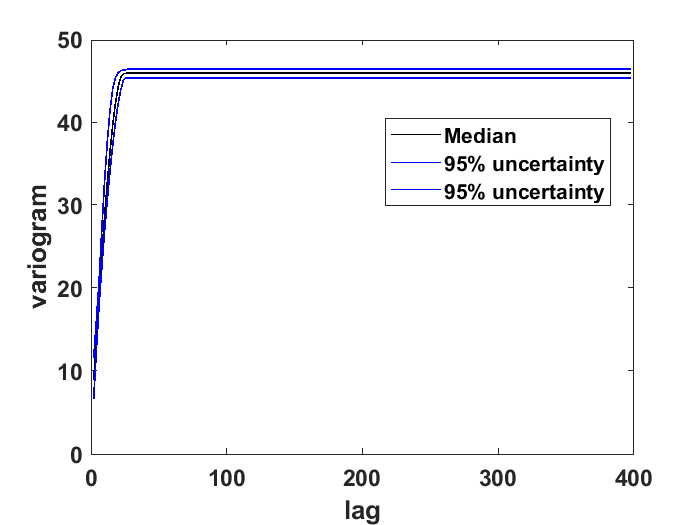
\includegraphics[width=0.55\columnwidth]{Q14_1.png} 
	\caption{Plot the experimental variogram with the median modeled variogram at each lag and 95\%
		uncertainty limits on the modeled variogram  }
\end{figure}

 \begin{figure}[htbp]
	\centering
	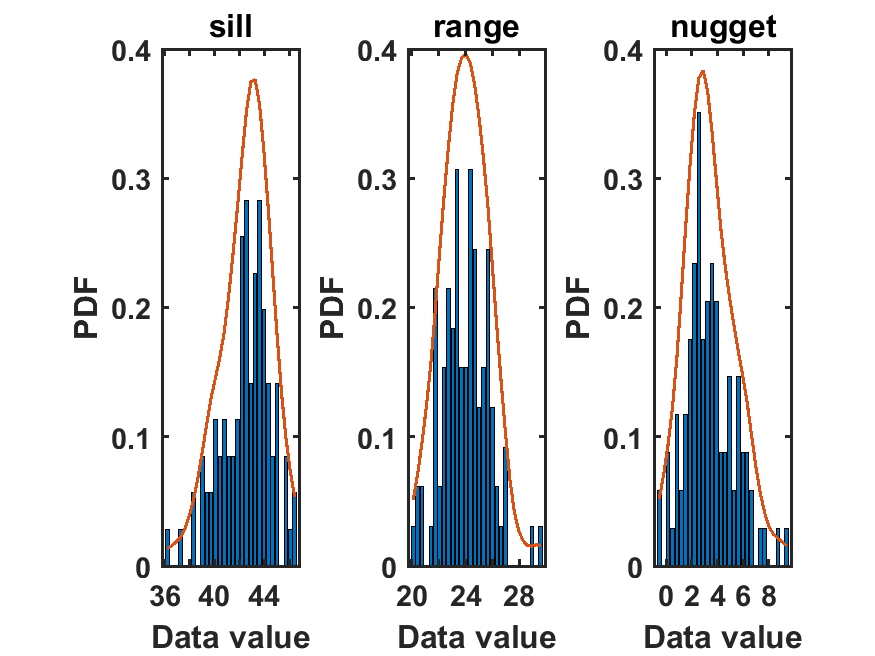
\includegraphics[width=.72\columnwidth]{Q14_2.png} 
	\caption{Plot the relative density histogram and kernel pdf for each of the variogram model parameters (sill, range, and nugget). }
\end{figure}


Codes
\begin{lstlisting}[language=Matlab,escapeinside=``]
%choose the spherical model with nugget which has smallest RMSE
np=150;%define the np
[h,psave,Vsave] = semivariogram_mc_model(x,y,np);%using new function to obtain the best parameters and variogram results

Vall=quantile(Vsave,[0.025 0.5 0.975]);% getmedian modeled variogram at each lag and 95% uncertainty limits
figure(11)
plot(h,Vall(2,:),'k','linewidth',1)% plot the median of semivariance 
hold on
plot(h,Vall(1,:),'b','linewidth',1)% plot the 95% uncertainty limits of semivariance
hold on
plot(h,Vall(3,:),'b','linewidth',1)% plot the 95% uncertainty limits of semivariance 
xlabel('lag')
ylabel('variogram')
legend('Median','95% uncertainty','95% uncertainty')
set(gca,'LineWidth',1,'FontSize',14,'FontWeight','bold')
print('Q14_1','-dpng')


bins=30;
h1=2;

figure(12)
subplot(1,3,1)
[centers] =plotRDH(psave(:,1),bins);%relative density histogram
hold on
[f] = myfun(psave(:,1),centers,h1); % do the Kernel estimation 
plot(centers,f,'LineWidth',1.5)  % plot the Kernel estimation 
title('sill')
set(gca,'LineWidth',1,'FontSize',14,'FontWeight','bold')


subplot(1,3,2)
[centers] =plotRDH(psave(:,2),bins);%relative density histogram
hold on
[f] = myfun(psave(:,2),centers,h1); % do the Kernel estimation 
plot(centers,f,'LineWidth',1.5)  % plot the Kernel estimation 
title('range')
set(gca,'LineWidth',1,'FontSize',14,'FontWeight','bold')


subplot(1,3,3)
[centers] =plotRDH(psave(:,3),bins);%relative density histogram
hold on
[f] = myfun(psave(:,3),centers,h1); % do the Kernel estimation 
plot(centers,f,'LineWidth',1.5)  % plot the Kernel estimation 
title('nugget')
set(gca,'LineWidth',1,'FontSize',14,'FontWeight','bold')

print('Q14_2','-dpng')

\end{lstlisting}
\end{document}
